\chapter{Test dei metodi di spam detection}
\lstset{basicstyle=\small\ttfamily,keywordstyle=\color{black}\bfseries,commentstyle=\color{darkgray},stringstyle=\color{black},showstringspaces=true} 
Nei capitoli precendenti sono stati illustrati vari metodi che di spam detection classificati basandosi sui segnali in ingresso che essi hanno bisogno per poter identificare le pagine web; quindi si hanno tre classi: metodi basati sul contenuto, metodi basati sul grafo e metodi che utilizzano segnali diversi dai primi due. Tra questi metodi ne sono stati presi in esame due: \textit{Trustrank} e \textit{Anti-trust rank}. 

Si è scelto, quindi, di valutare l'efficacia di due  algoritmi \textit{linked base} (\textit{Trustrank} e \textit{Anti-trust rank}) se essi operassero in modo online. Più precisamente i vari test consistono nel verificare quanto questi due algoritmi di tipo offline riescano ad approssimare il loro comportamento se li facessimo operare in modo online ovvero durante la fase di crawling. Le domande che ci poniamo eseguendo questi test su i due algoritmi di spam dection offline (\textit{Trustrank} e \textit{Anti-trus rank}) sono:
\begin{itemize}
 \item possono questi algoritmi essere in grado di operare in modalità online?
 \item durante l'esecuzione in modalità online, quanto riescono ad approssimare il loro comportamento offline?
 \item è conveniente utilizzare questi algoritmi in modalità online?
\end{itemize}

E' doveroso specificare che un algoritmo di spam detection lavora offline se questo viene eseguito dopo l'attività di crawling (e quindi dopo che si ha a disposizione l'intero grafo ottenuto dai collegamenti tra le pagine), mentre un algoritmo di spam detection lavora online se questo viene eseguito durante il processo di crawling e quindi riesce a determinare all'istante se una pagina deve essere considerata spam o non spam. Dal momento che si è scelto di esaminare degli algoritmi \textit{linked base}, e sapendo che questi formulano delle conclusioni sulla natura delle pagine (ovvero se sono spam o non spam) esaminando la struttura dell'intero grafo, è interessante notare come questi si comportino se il grafo su cui fare le valutazioni è incompleto.
%altre considerazioni

Il capitolo è diviso nel seguente modo: nella prima parte verrà illustrato come è stato scelto di simulare il crawler per poter eseguire gli algoritmi offline duratne la fase di crawling; nella seconda parte verrà spiegato come sono stati implementati i test; infine verrano illustrati tutti i test.

\section{Simulazione del crawler}
Per simulare il comportamento di crawler, e quindi eseguire gli algoritmi di \textit{Trustrank} e \textit{Anti-trust rank}, abbiamo implementato una semplice visita sul grafo in ampiezza ovvero una BFS \cite{bfsCormen} (Breadth-First Search). La visita in ampiezza dato un grafo \(G=(V,E)\), dove \(V\) è l'insieme dei vertici del grafo ed \(E\) l'insieme degli archi del grafo, e un vertice \(s\) da cui far partire la visita, scopre tutti i vertici che sono raggiungibili da \(s\). La visita in ampiezza scopre tutti i vertici che si trovano a distanza \(f\) dal vertice di partenza e successivamente scopre i vertici che si trovano a una distanza successiva \(f+1\). In sostanza dato il nodo di partenza \(s\), la visita in ampiezza, scopre tutti i nodi vicini al nodo \(s\) e successivamente per ogni nodo vicino scoperto trova i vicini che non sono ancora stati visitati; questo processo viene iterato finche tutti i nodi del grafo raggiungibili da \(s\) sono visitati. \\
Quindi anziche implementarci l'algoritmo BFS abbiamo utilizzato l'implementazione definita nel framework WebGraph. In particolare è stata utilizzata la classe ``ParallelBreadthFirstVisit'' che esegue una visita in ampiezza utilizzando il parallelismo derivato dai processori multicore.

\section{I test}
Come gia introdotto lo scopo dei test consiste che dato un algoritmo di spam detection che opera in modo offline valutare le sue prestazioni se operasse in modo online. Oltre tutto abbiamo scelto due algoritmi \textit{linked base} quali \textit{Trustrank} e \textit{Anti-trust rank} questo significa che l'algoritmo opererà su un grafo del web incompleto, all'inizio del crawling, fino ad arrivare ad operare sull'intero grafo alla fine del crawling.

\begin{figure}
\centering
 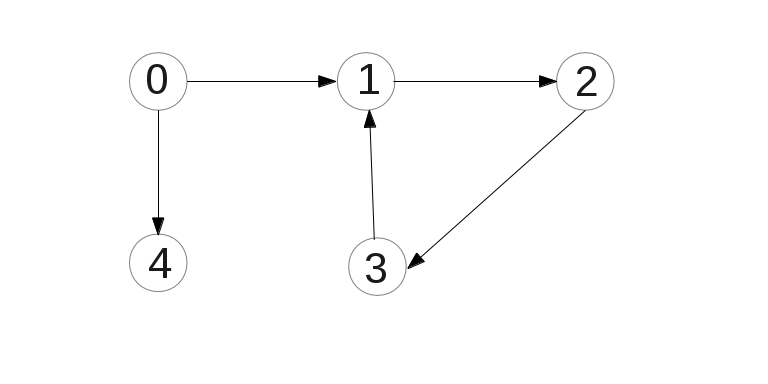
\includegraphics{immagini/test/grafoComp}
 \caption{Esempio di grafo}
 \label{fig:grafoComp}
\end{figure}

Quasi tutti i test seguono uno stesso schema; viene eseguito \textit{Trustrank} (e \textit{Anti-trust rank}) sul grafo completo, e lo indicheremo con \(t\) (\textit{Anti-trust rank} sarà indicato con \(a\)), successivamente viene eseguita la BFS (ovvero la visita in ampiezza) con nodo sorgente \(s\) e quindi si ricava la coda \(q\) dei nodi visitati a partire da \(s\); dopo di che si calcola \textit{Trustrank} (e \textit{Anti-trust rank}) sul grafo ricavati lungo la visita in ampiezza formato, quindi, da un sottoinsieme di nodi \(q\), il risultato lo indicheremo con \(\hat{t}_i\) (\textit{Anti-trust rank} sarà indicato con \(\hat{a}_i\)) dove \(i\) è il numero di nodi presi in considerazione dalla coda \(q\). Questo processo viene iterato incrementando sempre di più l'intervallo \(i\) finché non si arriva alla fine della coda \(q\) dei nodi visitati partendo dal nodo \(s\). Dopo aver calcolato \(t\) e \(\hat{t}_i\) sono due vettori si possono valutare tramite la Tau di Kendall e indicheremo con \(\tau(t,\hat{t}_i)\) la Tau di Kendall per \(t\) e \(\hat{t}_i\)  (e quindi \(\tau(a,\hat{a}_i)\) sarà la Tau di Kendall per \(a\) e \(\hat{a}_i\)). Ad esempio in figura \ref{fig:grafoComp} è rappresentato il grafo completo su cui verra calolato \(t\) e \(a\) mentre in figura \ref{fig:grafo3} è rappresentato il grafo ricavato dalla BFS eseguita sul grafo precedente partendo dal nodo 1; se si considerano tutti i nodi lungo la visita il vettore di \textit{trustrank} sarà \(\hat{t}_3\) mentre quello di \textit{anti-trust rank} sara \(\hat{a}_3\)..

 \begin{figure}
\centering
 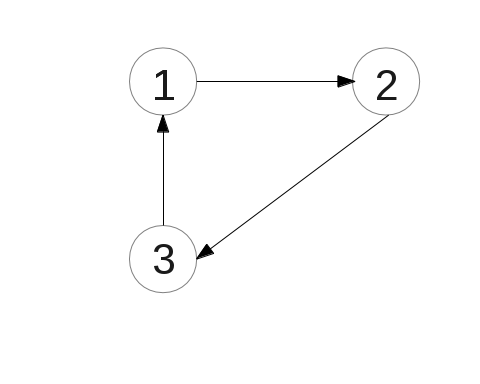
\includegraphics{immagini/test/grafo3}
 \caption{Esempio di grafo ricavato tramite una BFS a partire dal nodo 1 del grafo in figura \ref{fig:grafoComp}.}
 \label{fig:grafo3}
\end{figure}
A ogni indice del  vettore di \textit{Trustrank} \(t\) e del vettore di \textit{Anti-trust rank} \(a\) corrisponderà un nodo è il valore del vettore per un dato indice indica il valore di \textit{Trustrank} e \textit{Anti-trust rank} del nodo del grafo. In figura \ref{fig:tVettore} è illustrato un esempio del vettore di \textit{trustrank} calcolato sull'intero grafo e in figura \ref{fig:aVettore} è illustrato un esempio del vettore di \textit{anti-trust rank} calcolato sull'intero grafo. 
Nell'esempio in figura \ref{fig:tVettore} si nota che il vettore \(t\) di \textit{trustrank} ha lunghezza 5, quindi il grafo sarà composto da 5 nodi dove ad ogni nodo è associato il valore di \textit{trustrank}. Le stesse considerazioni valgono per l'esempio in figura \ref{fig:aVettore} dove il vettore di \textit{anti-trust rank} è ha lunghezza 5 e quindi l'algoritmo opererà su un grafo composto da 5 nodi.

\begin{figure}
\centering
 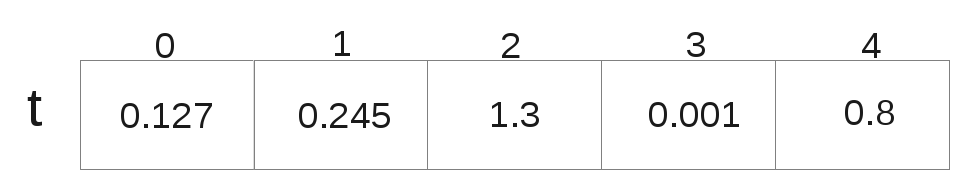
\includegraphics{immagini/test/trustVettore}
 \caption{Esempio del vettore di trustrank calcolato sull'intero grafo}
 \label{fig:tVettore}
\end{figure}
\begin{figure}
\centering
 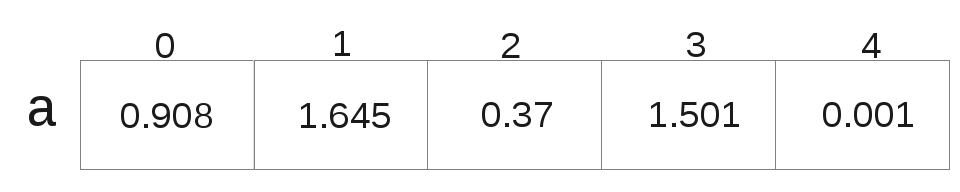
\includegraphics{immagini/test/immagineAntiTrust}
 \caption{Esempio del vettore di anti-trust rank calcolato sull'intero grafo}
 \label{fig:aVettore}
\end{figure}

A differenza dei vettori \(t\) e \(a\) (\textit{trustrank} eseguito sull'intero grafo e \textit{anti-trust rank} sull'intero grafo) , dove ad ogni indice (cioè ad ogni nodo) è associato un valore di \textit{trustrank} e \textit{anti-trust rank} , i vettori \(\hat{t}_i\) e \(\hat{a}_i\) non avranno per ogni indice un valore associato. Più precisamente, sapendo che \(\hat{t}_i\) e \(\hat{a}_i\) sono calcolati durante l'esecuzione di una BFS allora a ogni passo ci saranno ancora dei nodi da visitare per cui non è possibile calcolare i valori di \textit{trustrank} e \textit{anti-trust rank}. Quindi a ogni passo (quindi ogni qual volto vengono visitati un certo numero di nodi) sempre più nodi avranno associato un valore di \textit{trustrank} e \textit{anti-trust rank}, quindi \(\hat{t}_{i+1}\) avrà molti più nodi per cui è stato calcolato \textit{trustrank} rispetto a \(\hat{t}_i\) (questo vale anche per \textit{anti-trust rank}). Ma non è detto che dopo aver finalizzato la BFS partendo da un nodo \(s\) si sia visitato tutto il grafo (ovvero che \(s\) può raggiungere tutti i nodi del grafo) perciò in questo caso \(\hat{t}_i\) e \(\hat{a}_i\) avranno un numero minore di nodi per cui è calcolato \textit{trustrank} e \textit{anti-trust rank} rispetto a \(t\) e \(a\). Per gestire questa situazione i casi in cui gli indici non abbiano associato un valore ovvero quando la visita non ha ancora raggiunto tali nodi sono stati implementati due metodi.\\ 
Il primo metodo che chiameremo \textit{Modo\_A} assegna ad ogni indice dei vettori \(\hat{t}_i\) e \(\hat{a}_i\) non ancora visitato il valore 0.0. Ad esempio prendendo in considerazione il grafo in figura \ref{fig:grafoComp} e ipotizzando di eseguire una BFS a partire dal nodo 1 e di aver visitato i nodi 2 e 3 quindi se calcoliamo \textit{trustrank} e \textit{anti-trust rank} sul sottografo ricavato dai nodi visitati, i nodi 0 e 4 avranno associato i valori 0.0 (usando il metodo \textit{Modo\_A}), tale esempio è illustrato in figura \ref{fig:tBFSmodoA} e in figura \ref{fig:aBFSmodoA}.
\begin{figure}
\centering
 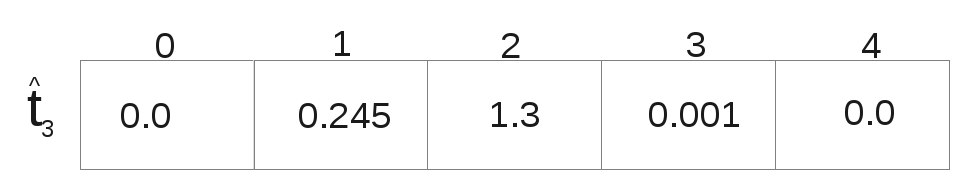
\includegraphics{immagini/test/tBFSmodoA}
 \caption{\textit{Modo\_A}. Esempio del vettore di trustrank calcolato su una porzione di grafo.}
 \label{fig:tBFSmodoA}
\end{figure}
\begin{figure}
\centering
 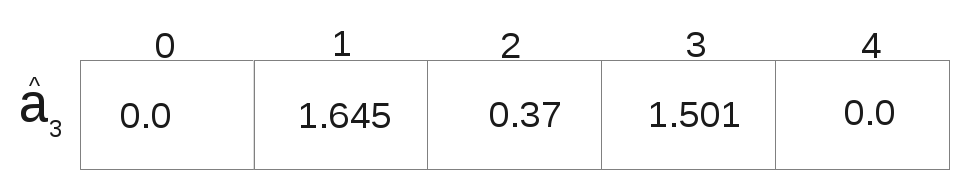
\includegraphics{immagini/test/aBFSmodoA}
 \caption{\textit{Modo\_A}. Esempio del vettore di anti-trust rank calcolato su una porzione di grafo.}
 \label{fig:aBFSmodoA}
\end{figure}
\\
Il secondo metodo che chiameremo \textit{Modo\_B} invece di assegnare il valore 0.0 ai nodi per cui non è possibile calcolare \textit{trustrank} e \textit{anti-trust rank} elimina tali indici dal vettore.  Ad esempio in figura \ref{fig:tBFSmodoB} viene illustrato il caso in cui eseguendo la BFS dal nodo 1, i nodi 0 e 4 rimangano senza aver assegnato un valore di \textit{trustrank}. Quindi gli indici 0 e 4 del vettore \(t\) non sono inclusi nel vettore \(\hat{t}_3\) questo implica che ci deve essere una corrispondenza tra gli indice del vettore \(t\) e quelli del vettore \(\hat{t}_3\) (in figura \ref{fig:tBFSmodoB} l'indice 0 del vettore \(\hat{t}_3\) corrisponde all'indice 1 del vettore \(t\), l'indice 1 al indice 2 ed infine l'indice 2 all'indice 3).  Si inoltre nota che il vettore \(\hat{t}_3\) ha lunghezza inferiore al vettore \(t\). 
\begin{figure}
\centering
 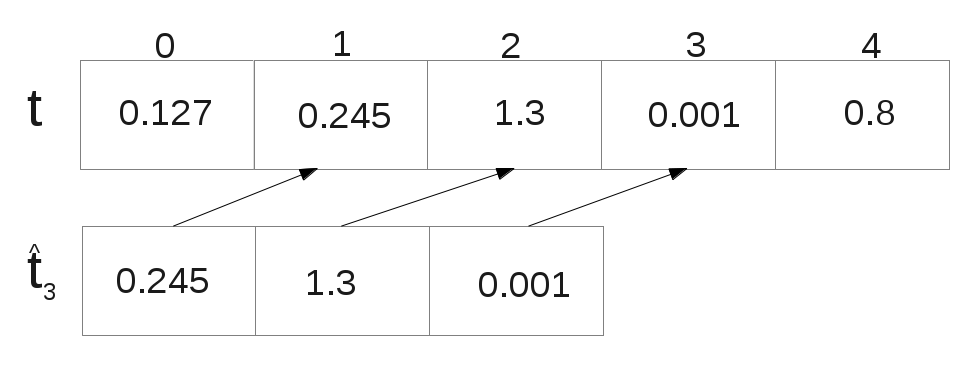
\includegraphics{immagini/test/tBFSmodoB}
 \caption{\textit{Modo\_B}. Esempio del vettore di trustrank calcolato su una porzione di grafo.}
 \label{fig:tBFSmodoB}
\end{figure}

Quindi la valutazione tra il vettore di \(t\), di \textit{trustrank}, calcolato sul grafo completo e il vettore \(\hat{t}_i\), di \textit{trustrank}, calcolato su una parte del grafo può avveniere usando ho il \textit{Modo\_A} o il \textit{Modo\_B}. Nel caso della valutazione nel \textit{Modo\_B} il vettore \(t\) dovra essere ristretto alla lunghezza del vettore \(\hat{t}_i\) e quindi dovranno essere eliminati gli indici del vettore \(t\) che non sono inclusi nel vettore \(\hat{t}_i\).
%parlare del fatto che al vettore d nel modoA bisogna togliere gli indici che non servono

I test saranno, quindi, cosi strutturari:
\begin{itemize}
 \item Test numero 1. Si confronta \textit{trustrank} sul grafo completo con \textit{trustrank} calcolato su una porzione di grafo. Lo stesso si fa per \textit{anti-trust ran}.
 \item Test numero 2. Si confrontano i solo nodi etichettati spam del vettore di  \textit{trustrank} sul grafo completo con  i soli nodi etichettati spam del vettore di \textit{trustrank} calcolato su una porzione di grafo. Nel caso di \textit{anti-trust rank} si  confrontano i nodi etichettati come non spam.
 \item Test numero 3. Si calcola \textit{trustrank} sul grafo completo ottenuto eseguendo la visita partendo da un nodo \(s\) e si confronta con \textit{trustrank} eseguito a ogni passo delle visita ma si imposta un seedset diverso formato dagli ultimi \(n\) nodi della vista. Viene applicato lo stesso metodo per \textit{anti-trust rank}.
 \item Test numero 4. Si esegue la BFS a partire dal nodo \(s\) e per ogni passo si calola la media dei valori di \textit{trustrank} dei soli nodi che sappiamo essere non spam e la media dei valori di \textit{Trustrank} dei soli nodi spam. Quindi si calcola la differenza tra le due medie. Lo stesso metodo verrà applicato per l'analisi dell'algoritmo di \textit{anti-trust rank}.
 \end{itemize}

 Dal momento che i test 1, 2 e 3 utilizzano la Tau di Kendall per calcolare la distanza tra i vettori \(t\) e \(\hat{t}_i\) allora ognuno dei test verra eseguito secondo il \textit{Modo\_A} e il \textit{Modo\_B}.
 
 \section{Test 1}
 Questo test calcola la distanza tra il vettore \(t\) di \textit{trustrank} ricavato sull'intero grafo e il vettore \(\hat{t}_i\) di \textit{trustrank} calcolato sul grafo ricavato dai nodi visitati lungo una visita in ampiezza con nodo sorgente \(s\). Inoltre viene eseguto lo stesso procedimento per quanto riguarda \textit{anti-trust rank} ovvero si calcolano le distanze tra il vettore di \(a\) di \textit{anti-trust rank} ottenuto dal grafo completo e il vettore \(\hat{a}_i\)  caloato sul grafo ricavato dai nodi visitati lungo  un visita in ampiezza con nodo sorgente \(s\).











